\documentclass[11pt]{article}
\usepackage{../emch574-homework}
\homeworknumber{02}
\studentname{J.C. Vaught}
\studentstatus{Graduate}
\duedate{TBD}
\begin{document}
\makehomeworktitle
\begingroup\small\sloppy\tableofcontents\endgroup
\newpage
\subsection*{Assignment}
\bulletitem{G signifies students that take this class for Graduate Credit; they must do all the items}
\bulletitem{UG students are not required to do the G work, but they may do it for bonus points}
\bulletitem{Problems solved beyond the minimum requirements will be given bonus points.}
\bulletitem{Challenge problems are optional; they will earn bonus points.}
\subsection*{Notes}
\bulletitem{Show your work to obtain partial credit if appropriate}
\bulletitem{Always display input data!}
\bulletitem{Partial credit might be given based on work done and MATLAB codes if they are attached; without them, no partial credit can be given.}
\bulletitem{Display numerical results to three significant digits (four if the first digit is 1).}
\bulletitem{Use SI system of measurement \href{https://en.wikipedia.org/wiki/International_System_of_Units}{reference}}
\bulletitem{Scale units using appropriate prefixes (e.g., nano, micro, milli, kilo, mega, giga, and so on) \href{https://en.wikipedia.org/wiki/Metric_prefix}{reference}}
\bulletitem{Problems solved beyond the minimum requirements will be given bonus points.}
\bulletitem{Challenge problems are optional. They may be solved for extra credit}
\bulletitem{Normalized plots are plots with the \ensuremath{y\text{-axis}} scaled between \ensuremath{-1} and \ensuremath{+1}. A plotted variable is normalized by dividing it by its maximum absolute value}
\subsubsection*{Notations and Abbreviations}
\bulletitem{BVP = boundary value problem}
\bulletitem{EOM = equation of motion}
\bulletitem{FBD = free body diagram}
\bulletitem{FRF = frequency response function}
\bulletitem{IVP = initial value problem}
\bulletitem{LHS = left hand side}
\bulletitem{NLM = Newton’s law of motion}
\bulletitem{ODE = ordinary differential equation}
\bulletitem{PDE = partial differential equation}
\bulletitem{RHS = right hand side}
\clearpage
\section{Waves}
\subsection{A.1 Wave Fundamentals}
\questionitem{1}{List at least five examples of waves met in everyday life}
\questionitem{2}{Explain in your own words the difference between disturbance waves and continuous waves}
\questionitem{3}{Explain using text and sketches the definition of wavespeed for a disturbance wave}
\questionitem{4}{Give at least three different equivalent expressions for a disturbance wave}
\questionitem{5}{A car pileup takes place on an interstate and propagates as a wave for several miles. What type of wave is this? Choose one of the following:}
\subquestionitem{a}{Continuous wave}
\subquestionitem{b}{Disturbance wave}
\questionitem{6}{Explain using text and sketches the definition of wavespeed for a continuous harmonic wave}
\questionitem{7}{Explain using text and sketches the definition of wavelength and wavenumber for a continuous harmonic wave}
\questionitem{8}{Give at least three different equivalent expressions for a continuous harmonic wave}
\questionitem{9}{What do waves carry? Choose one of the following:}
\subquestionitem{a}{Matter}
\subquestionitem{b}{Energy}
\subquestionitem{c}{Both}
\subquestionitem{d}{None of the above}
\questionitem{10}{Graduate work. Write about the particle-wave duality of light}
\clearpage
\subsection{A.2 Simple Wave Calculations}
Use the electromagnetic wavespeed \ensuremath{c_{\mathrm{light}}=300{,}000\,\mathrm{km}/\mathrm{s}} and sound wavespeed \ensuremath{c_{\mathrm{sound}}=340\,\mathrm{m}/\mathrm{s}}.

\taskprompt
\questionitem{1}{Calculate the frequency of visible light with typical wavelength \ensuremath{\lambda=510\,\mathrm{nm}}}
\questionitem{2}{Calculate the Hz frequency \ensuremath{f} of an AM radio wave with wavelength \ensuremath{\lambda=550\,\mathrm{m}}.}
\questionitem{3}{Infrared radiation has a typical wavelength \ensuremath{\lambda=10\,\mu\mathrm{m}}. What is the typical frequency of infrared radiation?}
\questionitem{4}{Calculate the wavelength \ensuremath{\lambda} of an FM radio wave with frequency \ensuremath{f=89\,\mathrm{MHz}}}
\questionitem{5}{The lightning flash is observed at \ensuremath{8{:}23{:}32\,\mathrm{p.m.}}, whereas the thunder is heard at \ensuremath{8{:}23{:}36\,\mathrm{p.m.}} How far away is the lightning strike? Give your answer in kilometers and miles}
\questionitem{6}{One of Verizon’s 5G mobile signals has frequency \ensuremath{f\approx29\,\mathrm{GHz}}. What is the corresponding wavelength?}
\questionitem{7}{A microwave oven typically operates at \ensuremath{f=2.5\,\mathrm{GHz}}}
\subquestionitem{a}{What is the wavelength \ensuremath{\lambda}?}
\subquestionitem{b}{What is the maximum permissible hole size \ensuremath{D} in the oven’s door mesh, given that the largest hole in a Faraday cage must be at most \ensuremath{\lambda/2}?}
\subquestionitem{c}{Measure approximately the hole size in a microwave oven door mesh and discuss your results. You may search the web for various opinions on this matter.}
\questionitem{8}{Graduate work. Given that the diameter of an electron is estimated to be \ensuremath{D=2\,\mathrm{pm}}, complete items (a) and (b)}
\subquestionitem{a}{Calculate the frequency of the electromagnetic wave that has a wavelength equal to the electron diameter}
\subquestionitem{b}{In what spectrum range would this electromagnetic wave be? (options: infrared, visible, ultraviolet, X-ray, gamma ray)}
\clearpage
\subsection{A.3 Calculate Car Motion on a Wavy Road}
Consider a car traveling on a wavy road. The road surface undulates with an amplitude \ensuremath{a=2.5\,\mathrm{in}} and a wavelength \ensuremath{\lambda=105\,\mathrm{ft}} that follows a cosine shape. The car is modeled as a spring-mass-damper (Figure~\ref{fig:hw02-01}) with natural frequency \ensuremath{f_{n}=0.95\,\mathrm{Hz}} and damping ratio \ensuremath{\zeta=22\%}. The maximum car speed is \ensuremath{v_{\mathrm{max}}=125\,\mathrm{mph}}.\par
\begin{figure}[H]
\centering
\setlength{\unitlength}{1pt}
\begin{picture}(301.85,139.15)
\put(0.00,0.00){
\includegraphics[width=301.85pt,height=139.15pt]{figures/extracted-000.png}}
\end{picture}
\caption{Car riding on a wavy road.}
\label{fig:hw02-01}
\end{figure}

\taskprompt
\questionitem{1}{Display input data}
\questionitem{2}{Calculate wavy road wavenumber \ensuremath{\gamma}}
\questionitem{3}{Plot the wavy road profile \ensuremath{u_{b}(x)} for \ensuremath{N_{\lambda}=2} wavelengths}
\questionitem{4}{Calculate wavy-road frequency \ensuremath{f_{\mathrm{max}}} for a maximum car speed of \ensuremath{v_{\mathrm{max}}} and define the frequency range \ensuremath{f=\operatorname{linspace}(0,f_{\mathrm{max}},N_{f})} with \ensuremath{N_{f}=2000}}
\questionitem{5}{Plot \ensuremath{\lvert \operatorname{FRF}(f;f_{n})\rvert}. Use datatips to locate the peak response and the matched-frequency response}
\questionitem{6}{Calculate the matched-frequency response value \ensuremath{\lvert \operatorname{FRF}_{n}\rvert}. Compare with the matched-frequency readings at item (5)}
\questionitem{7}{Calculate the car speed \ensuremath{v_{n}} needed to make wavy-road frequency \ensuremath{f} match the car natural frequency \ensuremath{f_{n}}}
\questionitem{8}{Use the conversion \ensuremath{f=v/\lambda} to plot \ensuremath{\lvert \operatorname{FRF}(v ; f_{n})\rvert}. Use datatips on the plot to find:}
\subquestionitem{a}{Find \ensuremath{v_{n}} and \ensuremath{\lvert \operatorname{FRF}_{n}\rvert}, and compare them with the results of items (6) and (7)}
\subquestionitem{b}{Find \ensuremath{v_{\mathrm{cr}}} and \ensuremath{\lvert \operatorname{FRF}_{\mathrm{max}}\rvert}}
\subquestionitem{c}{The limit speed \ensuremath{v_{\mathrm{limit}}} for which the motion amplification is limited to \ensuremath{\lvert \operatorname{FRF}_{\mathrm{lim}}\rvert =1.5}}
\questionitem{9}{Graduate work. Find the road wavelength \ensuremath{\lambda_{\mathrm{new}}} that will make \ensuremath{v_{n}=35\,\mathrm{mph}}}
\questionitem{10}{Graduate work. Repeat items (5) through (8) for a car with worn-out shocks that provide only \ensuremath{\zeta=10\%}, and compare the two cases}
\clearpage
\subsection{A.4 Standing Waves}
\questionitem{1}{Follow the notes to develop the standing-wave concept:}
\subquestionitem{a}{Write the complex-exponential expressions for two identical harmonic waves of amplitude \ensuremath{1/2} propagating in opposite directions}
\subquestionitem{b}{Add the two waves and write the resulting complex-exponential expression}
\subquestionitem{c}{Use Euler’s formula to arrive at a trigonometric expression}
\questionitem{2}{Sketch a standing wave and identify the nodes and antinodes (bows)}
\questionitem{3}{Assume wavespeed \ensuremath{c=340\,\mathrm{m}/\mathrm{s}} and frequency \ensuremath{f=2.9\,\mathrm{kHz}}. Calculate:}
\subquestionitem{a}{Rad/sec frequency \ensuremath{\omega}}
\subquestionitem{b}{Wavenumber \ensuremath{\gamma}}
\subquestionitem{c}{Wavelength \ensuremath{\lambda}}
\subquestionitem{d}{Distance \ensuremath{\Delta x} between standing wave nodes}
\questionitem{4}{Graduate work. Explain intuitively the analogy between standing waves and the vibration of a taut string}
\clearpage
\subsection{A.5 Musical Notes}
\questionitem{1}{Find the Hz frequency of note \ensuremath{C_{5}}}
\questionitem{2}{Find what musical note corresponds to \ensuremath{246.94\,\mathrm{Hz}}}
\questionitem{3}{What is the lowest frequency on the scale of equal temperament and what musical note does it correspond to?}
\questionitem{4}{What is the commonly accepted frequency range of human hearing?}
\questionitem{5}{What is the highest frequency on the scale of equal temperament and what musical note does it correspond to?}
\questionitem{6}{Graduate work. Explain the scale of equal temperament by answering items (a)--(c)}
\subquestionitem{a}{What is the organizing principle of the scale of equal temperament}
\subquestionitem{b}{How many equal-temperament entries are in an octave?}
\subquestionitem{c}{What is the ratio between two adjacent entries on the scale of equal temperament?}
\clearpage
\subsection{A.6 Musical Instruments}
\questionitem{1}{List at least three methods to produce sound in a string instrument}
\questionitem{2}{List the two different methods to produce a sound in wind instruments}
\questionitem{3}{List string instruments that use a hammer hit to produce sound}
\questionitem{4}{List the three major categories of musical instruments. For each category, complete items (a) and (b)}
\subquestionitem{a}{Describe how the instrument works}
\subquestionitem{b}{Explain what physical principles are used to produce sound}
\questionitem{5}{List at least five common string instruments}
\clearpage
\section{Fluid Waves and Vibration}
\subsection{B.1 Analyze the Wave Equation in Fluids}
\begin{figure}[H]
\centering
\setlength{\unitlength}{1pt}
\begin{picture}(324.00,63.90)
\put(0.00,0.00){
\includegraphics[width=324.00pt,height=63.90pt]{figures/extracted-005.png}}
\end{picture}
\caption{Fluid waves in an infinite tube.}
\label{fig:hw02-02}
\end{figure}
Assume an infinite tube of cross section \ensuremath{A} containing fluid of density \ensuremath{\rho} and bulk modulus \ensuremath{K} (Figure~\ref{fig:hw02-02}). Develop the wave equation in fluids.

\taskprompt
\questionitem{1}{Assume that the fluid in the tube undergoes time-varying axial displacement \ensuremath{u(x,t)} under the influence of a pressure disturbance \ensuremath{p(x,t)}}
\questionitem{2}{Consider an infinitesimal element \ensuremath{d x} and draw the displacements and pressures on both of its sides}
\questionitem{3}{Draw FBD}
\questionitem{4}{Apply NLM and deduce relationship between pressure \ensuremath{p}, density \ensuremath{\rho} and acceleration \ensuremath{\ddot{u}}}
\questionitem{5}{Apply fluid-elasticity equation and express the pressure \ensuremath{p(x,t)} in terms of displacement \ensuremath{u(x,t)} and bulk modulus \ensuremath{K}}
\questionitem{6}{Substitute (5) into (4) and deduce the relationship between the second derivative with respect to space, \ensuremath{u''}, and the second derivative with respect to time, \ensuremath{\ddot{u}}}
\questionitem{7}{Define the wavespeed \ensuremath{c}}
\questionitem{8}{Substitute (7) into (6) and deduce the wave equation}
\clearpage
\subsection{B.2 Analyze and Solve the Wave Equation}
Recall the results of Problem B.1.

\taskprompt
\questionitem{1}{Recall the wave equation}
\questionitem{2}{Assume separation of time and space behaviors into \ensuremath{U(x)} and \ensuremath{T(t)} and write \ensuremath{u(x,t)} as a function of \ensuremath{U(x)} and \ensuremath{T(t)}}
\questionitem{3}{Perform the appropriate differentiations with respect to space and time}
\questionitem{4}{Assume vibratory time behavior with angular frequency \ensuremath{\omega} using a complex exponential formula for \ensuremath{T(t)}}
\questionitem{5}{Substitute (4) into (3) and write expressions for \ensuremath{u''} and \ensuremath{\ddot{u}}}
\questionitem{6}{Substitute (5) into the wave equation (1) and express it only in terms of \ensuremath{U(x)}, \ensuremath{c}, \ensuremath{\omega}}
\questionitem{7}{Define wavenumber \ensuremath{\gamma}}
\questionitem{8}{Substitute (7) into (6) and obtain a linear ordinary differential equation (ODE) in terms of \ensuremath{U(x)}, \ensuremath{U''(x)}, and \ensuremath{\gamma}}
\questionitem{9}{Assume exponential solution of the form \ensuremath{U(x)=e^{s x}}}
\questionitem{10}{Substitute (9) into (8) and obtain the characteristic equation}
\questionitem{11}{Solve the characteristic equation (10) and obtain the roots \ensuremath{s_{1}}, \ensuremath{s_{2}}}
\questionitem{12}{Substitute (11) into (9) and write the complete solution in terms of constants \ensuremath{A_{1}}, \ensuremath{A_{2}} and complex exponentials of \ensuremath{s_{1}}, \ensuremath{s_{2}}}
\questionitem{13}{Add the vibratory time behavior from (4) to obtain the solution in terms of complex exponentials depending on both \ensuremath{\gamma} and \ensuremath{\omega}}
\questionitem{14}{Use Euler’s formulas to rewrite (13) in terms of new constants \ensuremath{C_{1}} and \ensuremath{C_{2}}, trigonometric functions depending on \ensuremath{\gamma}, and a complex exponential depending on \ensuremath{\omega}}
\clearpage
\subsection{B.3 Analyze Air Vibration in a Tube Closed at Both Ends}
\begin{figure}[H]
\centering
\setlength{\unitlength}{1pt}
\begin{picture}(316.39,97.25)
\put(0.00,0.00){
\includegraphics[width=316.39pt,height=97.25pt]{figures/extracted-008.png}}
\end{picture}
\caption{Air vibration in a tube of finite length \ensuremath{L} closed at both ends.}
\label{fig:hw02-03}
\end{figure}
Assume a tube of finite length \ensuremath{L} and cross section \ensuremath{A} containing fluid of density \ensuremath{\rho}, bulk modulus \ensuremath{K}, and wavespeed \ensuremath{c} (Figure~\ref{fig:hw02-03}). The tube is closed at both ends. The air in the tube undergoes harmonic axial displacement \ensuremath{u(x,t)} with frequency \ensuremath{\omega}.

\taskprompt
\questionitem{1}{Write the boundary conditions at the two ends of the tube in terms of displacement \ensuremath{u(x,t)}}
\questionitem{2}{Recall the harmonic solution of the wave equation consisting of the multiplication of two terms:}
\subquestionitem{a}{First term: a function \ensuremath{U(x)} consisting of trigonometric functions depending on wavenumber \ensuremath{\gamma}, space variable \ensuremath{x}, and constants \ensuremath{C_{1}}, \ensuremath{C_{2}}}
\subquestionitem{b}{Second term: a complex exponential depending on frequency \ensuremath{\omega} and time variable \ensuremath{t}}
\questionitem{3}{Substitute (2) into (1) and write the boundary conditions at the two ends of the tube in terms of unknown constants \ensuremath{C_{1}}, \ensuremath{C_{2}}}
\questionitem{4}{Solve (3) for \ensuremath{C_{2}} and obtain an equation for \ensuremath{C_{1}}}
\questionitem{5}{Discuss the trivial solution}
\questionitem{6}{Choose to search for the nontrivial solution and define the equation that needs to be solved to find a nontrivial solution}
\questionitem{7}{Introduce the notation \ensuremath{z=\gamma L} into (6) and write the eigenvalue equation in terms of \ensuremath{z}}
\questionitem{8}{Solve the eigenvalue equation and write the general expression for the eigenvalues \ensuremath{z_{j}}, where \ensuremath{j=1,2,3,\ldots}}
\questionitem{9}{Use (7) to write the general expression for the wavenumber \ensuremath{\gamma} in terms of \ensuremath{j} and length \ensuremath{L}}
\questionitem{10}{Recall from HW01 the definition of wavenumber \ensuremath{\gamma} in terms of frequency \ensuremath{\omega} and wavespeed \ensuremath{c}}
\questionitem{11}{Solve (10) for frequency \ensuremath{\omega} in terms of wavenumber \ensuremath{\gamma} and wavespeed \ensuremath{c}}
\questionitem{12}{Use (9) and (11) to write the general expression of the natural frequency \ensuremath{\omega_{j}} in terms of \ensuremath{j}, wavespeed \ensuremath{c}, and tube length \ensuremath{L}}
\questionitem{13}{Use (12) to write the general expression of the Hz frequency \ensuremath{f} in terms of \ensuremath{j}, wavespeed \ensuremath{c}, and tube length \ensuremath{L}}
\questionitem{14}{Explain the meaning of fundamental frequency and overtones}
\questionitem{15}{Explain the meaning of fundamental harmonic and higher harmonics}
\questionitem{16}{Recall the relationship between wavelength \ensuremath{\lambda} and wavenumber \ensuremath{\gamma}}
\questionitem{17}{Substitute (9) into (16) to write the general expression for the wavelength \ensuremath{\lambda_{j}} in terms of \ensuremath{j} and tube length \ensuremath{L}}
\questionitem{18}{Use (17) to explain which wavelength multiples could accommodate vibratory standing waves in a tube of length \ensuremath{L} closed at both ends}
\questionitem{19}{Recall \ensuremath{U(x)} from (2)(a) and use (4) to eliminate \ensuremath{C_{2}}}
\questionitem{20}{Set \ensuremath{C_{1}=1} in item (19) and write the general expression for the displacement modeshape \ensuremath{U_{j}(x)} in terms of the wavenumber \ensuremath{\gamma_{j}}}
\questionitem{21}{Write the general expression of the pressure modeshapes}
\clearpage
\subsection{B.4 Calculate Air Vibration in a Tube Closed at Both Ends}
Consider a tube of length \ensuremath{L=0.85\,\mathrm{m}} closed at both ends. Take sound speed \ensuremath{c=340\,\mathrm{m}/\mathrm{s}} and air density \ensuremath{\rho=1.2\,\mathrm{kg}/\mathrm{m}^{3}}. Use the results of Problem B.3 to calculate the modal vibration characteristics and modeshapes for \ensuremath{j=1,\ldots,N} with \ensuremath{N=5}.\par
\questionitem{1}{Display input data}
\questionitem{2}{Calculate and display the modal vibration characteristics:}
\subquestionitem{a}{Eigenvalues \ensuremath{z_{j}}}
\subquestionitem{b}{Wavenumbers \ensuremath{\gamma_{j}}}
\subquestionitem{c}{Rad/s frequencies \ensuremath{\omega_{j}}}
\subquestionitem{d}{Hz frequencies \ensuremath{f_{j}}}
\questionitem{3}{Calculate and plot the displacement modeshapes}
\questionitem{4}{Discuss your results}
\questionitem{5}{Graduate work. Calculate and plot the normalized pressure modeshapes, and compare the result with item (3)}
\clearpage
\subsection{B.5 Calculate the Slide Whistle}
Consider the slide whistle shown in Figure~\ref{fig:hw02-04}. The fully retracted whistle is shown in Figure~\ref{fig:hw02-04}(a), whereas the fully extended whistle is shown in Figure~\ref{fig:hw02-04}(b). The length of the residual cavity of the fully retracted whistle tube can be approximated to be \ensuremath{L_{0} = 6\,\mathrm{mm}} (Figure~\ref{fig:hw02-04}(a)). The thickness of the piston inside the whistle can be approximated to be \ensuremath{L_{p} = 6\,\mathrm{mm}}. The thickness of the end walls can be approximated to be \ensuremath{L_{w} = 6\,\mathrm{mm}}. Assume sound speed in air to be \ensuremath{c=340\,\mathrm{m}/\mathrm{s}}. The purpose of this problem is to calculate the fundamental frequency for various positions of the whistle slider\par
\begin{figure}[H]
\centering
\setlength{\unitlength}{1pt}
\begin{picture}(307.71,207.48)
\put(1.85,119.43){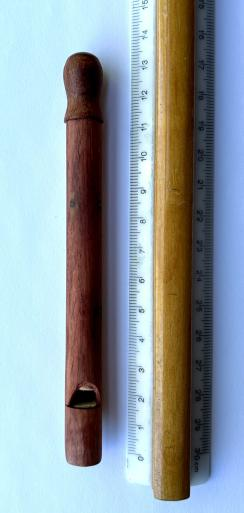
\includegraphics[width=184.70pt,height=88.05pt]{figures/extracted-009.png}}
\put(0.00,0.00){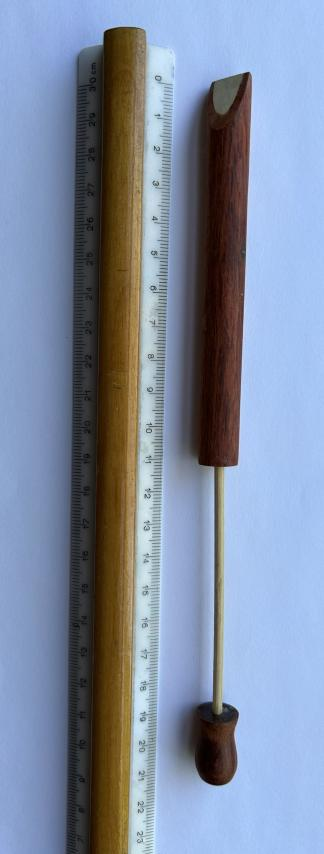
\includegraphics[width=307.71pt,height=116.75pt]{figures/extracted-010.png}}
\end{picture}
\caption{Slide whistle. (a) Fully retracted, showing the piston end. (b) Fully extended. The ruler's major markings are in centimeters.}
\label{fig:hw02-04}
\end{figure}
Recall the theoretical results of Problem B.3.

\taskprompt
\questionitem{1}{Display input data}
\questionitem{2}{Use Figure~\ref{fig:hw02-04} to estimate the fully extended whistle length \ensuremath{L_{e}}}
\questionitem{3}{Use Figure~\ref{fig:hw02-04} to estimate the fully contracted whistle length \ensuremath{L_{c}}}
\questionitem{4}{Use \ensuremath{L_{e}}, \ensuremath{L_{c}} to calculate the extension travel \ensuremath{dL_{I}} corresponding to fully extended slide whistle}
\questionitem{5}{Use \ensuremath{dL_{I}} and \ensuremath{L_{0}} to calculate the cavity length \ensuremath{L_{I}} of a fully extended slide whistle}
\questionitem{6}{Estimate the fully extended frequency \ensuremath{f_{I}} in Hz and find the nearest musical note expressed as a letter name and octave number (e.g., \ensuremath{\mathrm{G3}} signifies note G in the third octave)}
\questionitem{7}{Use \ensuremath{L_{e}}, \ensuremath{L_{c}} to calculate the extension travel \ensuremath{dL_{\mathrm{II}}} corresponding to \ensuremath{40\%} extended slide whistle}
\questionitem{8}{Use \ensuremath{dL_{\mathrm{II}}} and \ensuremath{L_{0}} to calculate the cavity length \ensuremath{L_{\mathrm{II}}} of a \ensuremath{40\%}-extended slide whistle}
\questionitem{9}{Calculate the \ensuremath{40\%}-extended frequency \ensuremath{f_{\mathrm{II}}} in Hz and find the nearest musical note expressed as a letter name and an octave number}
\questionitem{10}{Comment on your work}
\subsubsection*{Graduate Work}
Estimate the piston position required to obtain the musical note \ensuremath{\mathrm{B7}}.

\taskprompt
\questionitem{11}{Display the frequency \ensuremath{f_{\mathrm{III}}} of the note \ensuremath{\mathrm{B7}}}
\questionitem{12}{Calculate the cavity length \ensuremath{L_{\mathrm{III}}} needed to generate frequency \ensuremath{f_{\mathrm{III}}} of the note \ensuremath{\mathrm{B7}}}
\questionitem{13}{Calculate the extension travel \ensuremath{dL_{\mathrm{III}}} needed to generate frequency \ensuremath{f_{\mathrm{III}}} of the note \ensuremath{\mathrm{B7}}}
\questionitem{14}{Estimate what percentage of the piston must be extended to generate the note \ensuremath{\mathrm{B7}}}
\questionitem{15}{Comment on your work}
\clearpage
\subsection{B.6 Calculate Sound Intensity and the dB Scale}
Take sound speed \ensuremath{c=340\,\mathrm{m}/\mathrm{s}} and air density \ensuremath{\rho=1.2\,\mathrm{kg}/\mathrm{m}^{3}}.

\taskprompt
\questionitem{1}{Display input data}
\questionitem{2}{Calculate air’s acoustic impedance \ensuremath{Z}}
\questionitem{3}{Calculate the sound intensity \ensuremath{I} corresponding to a sound pressure \ensuremath{p=55\,\mathrm{mPa}}}
\questionitem{4}{Give the values of the reference sound intensity \ensuremath{I_{0}} and reference sound pressure \ensuremath{p_{0}}}
\questionitem{5}{Convert the sound pressure and sound intensity from item (3) to decibels}
\questionitem{6}{Verify that the sound pressure and sound intensity calculated at item (5) have the same dB value and explain why it is so}
\questionitem{7}{Calculate in physical units the sound intensity, sound pressure, and sound power from a loudspeaker with diameter \ensuremath{D=1.55\,\mathrm{m}} working at \ensuremath{78\,\mathrm{dB}}}
\questionitem{8}{Calculate the sound pressure \ensuremath{p_{\mathrm{horn}}} created by a \ensuremath{118\,\mathrm{dB}} car horn}
\questionitem{9}{Give the values of the pain sound intensity \ensuremath{I_{\mathrm{pain}}} and pain sound pressure \ensuremath{p_{\mathrm{pain}}} and comment on the results of items (7) and (8) relative to pain values}
\questionitem{10}{Graduate work. Explain why different decibel-conversion formulas are required for sound intensity \ensuremath{I} and sound pressure \ensuremath{p}}
\clearpage
\section{Extra Credit Challenge Problems}
Challenge problems are optional.\par
\subsection{C.1 Analyze Air Vibration in a Closed-Open Tube}
\questionitem{1}{Sketch a tube closed at one end and open at the other end indicating all the information needed for the analysis}
\questionitem{2}{Write the boundary conditions at the two ends of the tube in terms of displacement \ensuremath{u(x,t)} and pressure disturbance \ensuremath{p(x,t)}}
\questionitem{3}{Recall from HW01 the harmonic solution of the wave equation consisting of the multiplication of two terms:}
\subquestionitem{a}{First term: a function \ensuremath{U(x)} consisting of trigonometric functions depending on wavenumber \ensuremath{\gamma}, space variable \ensuremath{x}, and constants \ensuremath{C_{1}}, \ensuremath{C_{2}}}
\subquestionitem{b}{Second term: a complex exponential depending on frequency \ensuremath{\omega} and time variable \ensuremath{t}}
\questionitem{4}{Recall from HW01 the expression of pressure \ensuremath{p(x,t)} in terms of displacement \ensuremath{u(x,t)} and bulk modulus \ensuremath{K}}
\questionitem{5}{Substitute (3) into (4) to obtain the pressure \ensuremath{p(x,t)} in terms of constants \ensuremath{C_{1}}, \ensuremath{C_{2}}}
\questionitem{6}{Substitute (3) and (5) into (2) and write the boundary conditions at the two ends of the tube in terms of unknown constants \ensuremath{C_{1}}, \ensuremath{C_{2}}}
\questionitem{7}{Solve (6) for \ensuremath{C_{2}} and obtain an equation for \ensuremath{C_{1}}}
\questionitem{8}{Discuss the trivial solution}
\questionitem{9}{Choose to search for the nontrivial solution and define the equation that needs to be solved to find a nontrivial solution}
\questionitem{10}{Introduce the notation \ensuremath{z=\gamma L} into (9) and write the eigenvalue equation in terms of \ensuremath{z}}
\questionitem{11}{Solve the eigenvalue equation and write the general expression for the eigenvalues \ensuremath{z_{j}}, where \ensuremath{j=1,2,3,\ldots}}
\questionitem{12}{Use (10) to write the general expression for the wavenumber \ensuremath{\gamma_{j}} in terms of \ensuremath{j} and length \ensuremath{L}}
\questionitem{13}{Recall from HW01 the definition of wavenumber \ensuremath{\gamma} in terms of frequency \ensuremath{\omega} and wavespeed \ensuremath{c}}
\questionitem{14}{Solve (13) for frequency \ensuremath{\omega} in terms of wavenumber \ensuremath{\gamma} and wavespeed \ensuremath{c}}
\questionitem{15}{Use (12) and (14) to write the general expression of the natural frequency \ensuremath{\omega_{j}} in terms of \ensuremath{j}, wavespeed \ensuremath{c}, and tube length \ensuremath{L}}
\questionitem{16}{Use (15) to write the general expression of the Hz frequency \ensuremath{f_{j}} in terms of \ensuremath{j}, wavespeed \ensuremath{c}, and tube length \ensuremath{L}}
\questionitem{17}{Explain the meaning of fundamental frequency and overtones}
\questionitem{18}{Explain the meaning of fundamental harmonic and higher harmonics}
\questionitem{19}{Recall from HW01 the relationship between wavelength \ensuremath{\lambda} and wavenumber \ensuremath{\gamma}}
\questionitem{20}{Substitute (12) into (19) to write the general expression for the wavelength \ensuremath{\lambda_{j}} in terms of \ensuremath{j} and tube length \ensuremath{L}}
\questionitem{21}{Use (20) to explain which wavelength multiples could accommodate vibratory standing waves in a tube of length \ensuremath{L} closed at one end and open at the other end}
\questionitem{22}{Recall \ensuremath{U(x)} from (3)(a) and use (7) to eliminate \ensuremath{C_{2}}}
\questionitem{23}{Set \ensuremath{C_{1}=1} in item (22) and write the general expression for the modeshape \ensuremath{U_{j}(x)} in terms of the wavenumber \ensuremath{\gamma_{j}}}
\questionitem{24}{Plot the normalized displacement modeshapes for modes 1 through 5 of air vibration in a tube of length \ensuremath{L}, and discuss your results}
\questionitem{25}{Graduate work. Calculate and plot the normalized pressure modeshapes for modes 1 through 5 of air vibration in a tube of length \ensuremath{L}, and discuss your results}
\clearpage
\subsection{C.2 Analyze Air Vibration in an Open-Open Tube}
\questionitem{1}{Sketch a tube open at both ends indicating the information needed for analysis}
\questionitem{2}{Write the boundary conditions at the two ends of the tube}
\questionitem{3}{Repeat all steps of Problem C.1 paying particular attention to the values taken by \ensuremath{C_{1}} and \ensuremath{C_{2}}}
\clearpage
\subsection{C.3 Calculate Air Vibration in a Tube with Various Boundary Conditions}
Consider a tube of length \ensuremath{L=0.85\,\mathrm{m}}. Take sound speed \ensuremath{c=340\,\mathrm{m}/\mathrm{s}} and air density \ensuremath{\rho=1.2\,\mathrm{kg}/\mathrm{m}^{3}}. The purpose is to calculate the modal vibration characteristics and modeshapes for \ensuremath{j=1,\ldots,N} with \ensuremath{N=5}. The following boundary conditions are considered.\par
\begin{center}
\begin{tabular}{@{}cll@{}}
\toprule
Case & \ensuremath{x=0} & \ensuremath{x=L} \\
\midrule
(i) & Closed & Open \\
(ii) & Open & Open \\
\bottomrule
\end{tabular}
\end{center}
\questionitem{1}{Display the input data}
\instruction{For each boundary-condition case, complete items (2)--(5)}
\questionitem{2}{Calculate and display the modal vibration characteristics:}
\subquestionitem{a}{Eigenvalues \ensuremath{z_{j}}}
\subquestionitem{b}{Wavenumbers \ensuremath{\gamma_{j}}}
\subquestionitem{c}{Rad/s frequencies \ensuremath{\omega_{j}}}
\subquestionitem{d}{Hz frequencies \ensuremath{f_{j}}}
\questionitem{3}{Calculate and plot the displacement modeshapes}
\questionitem{4}{Compare your results with those of Problem B.4}
\questionitem{5}{Graduate work. Calculate and plot the normalized pressure modeshapes, and compare the result with item (3)}
\end{document}
